\documentclass{article}

% set font encoding for PDFLaTeX or XeLaTeX
\usepackage{graphicx}
\usepackage{ifxetex}
\ifxetex
  \usepackage{fontspec}
\else
  \usepackage[T1]{fontenc}
  \usepackage[utf8]{inputenc}
  \usepackage{lmodern}
\fi

% used in maketitle
\title{Evaluacion 2}
\author{Corral Valdez Jesus Giovanni\\
Departamento de Fisica \\
Universidad de Sonora}
\date{01 de diciembre de 2017}


% Enable SageTeX to run SageMath code right inside this LaTeX file.
% documentation: http://mirrors.ctan.org/macros/latex/contrib/sagetex/sagetexpackage.pdf
% \usepackage{sagetex}

\begin{document}
\maketitle
\clearpage

\section{Actividad 1: Describir el ejemplo}
El programa del ejemplo, se le da un valor "n" y "x" ya escogidos (20 y 1.0 respectivamente). Con estos datos se calcula mediante una Serie de Maclaurin el exponencial del valor de x en una funcion. En el programa se llama a esa funcion otorgandole los valores ya elegidos y te arroja el resultado del exponencial calculado, pero tambien el programa te imprimi el exponencial verdadero con el comando de "exp(x)" y ya se compara el error entre el exponencial que calculamos en la función que es muy aproximado (si se hubiera hecho mas iteraciones seria aun mas aproximado).

\clearpage
\section{Actividad 2: Exponente}
\begin{verbatim}
subroutine exptaylor (n, j, fi, fj, exptay)
	integer, intent (in)      :: n
	double precision, intent (in) :: fi
	integer :: j
	double precision, dimension (100), intent(out) :: exptay
	double precision :: fj, term, partial_sum
	
	
	
	term = 1
	partial_sum = term
	do j = 1, n
	 fj = dble(j)
	 term = term * fi / fj
	 partial_sum = partial_sum + term
	 exptay(j) = partial_sum
	enddo

	 
end subroutine exptaylor
	 

program segundo
	double precision, dimension (15) :: f
	integer :: i, j, n
	double precision, dimension (100)   :: x
	double precision, dimension (100) :: exptay
	double precision, dimension (100) :: funcion
	double precision :: fi, fj, term, partial_sum

     open (1, file = 'datos.dat', status = 'unknown')
	
	do n=1, 15, 2
	do i=0, 100, 1
	  fi = dble(i)
	  fi = fi / 10.0d0
	call exptaylor (n, j, fi, fj, exptay)
	funcion(n) = exptay(n)
	write (1,*) fi, funcion(n)

	end do
	write (1,*) ' '
	end do
     close (1)

end program segundo
\end{verbatim}
\clearpage
\begin{figure}
  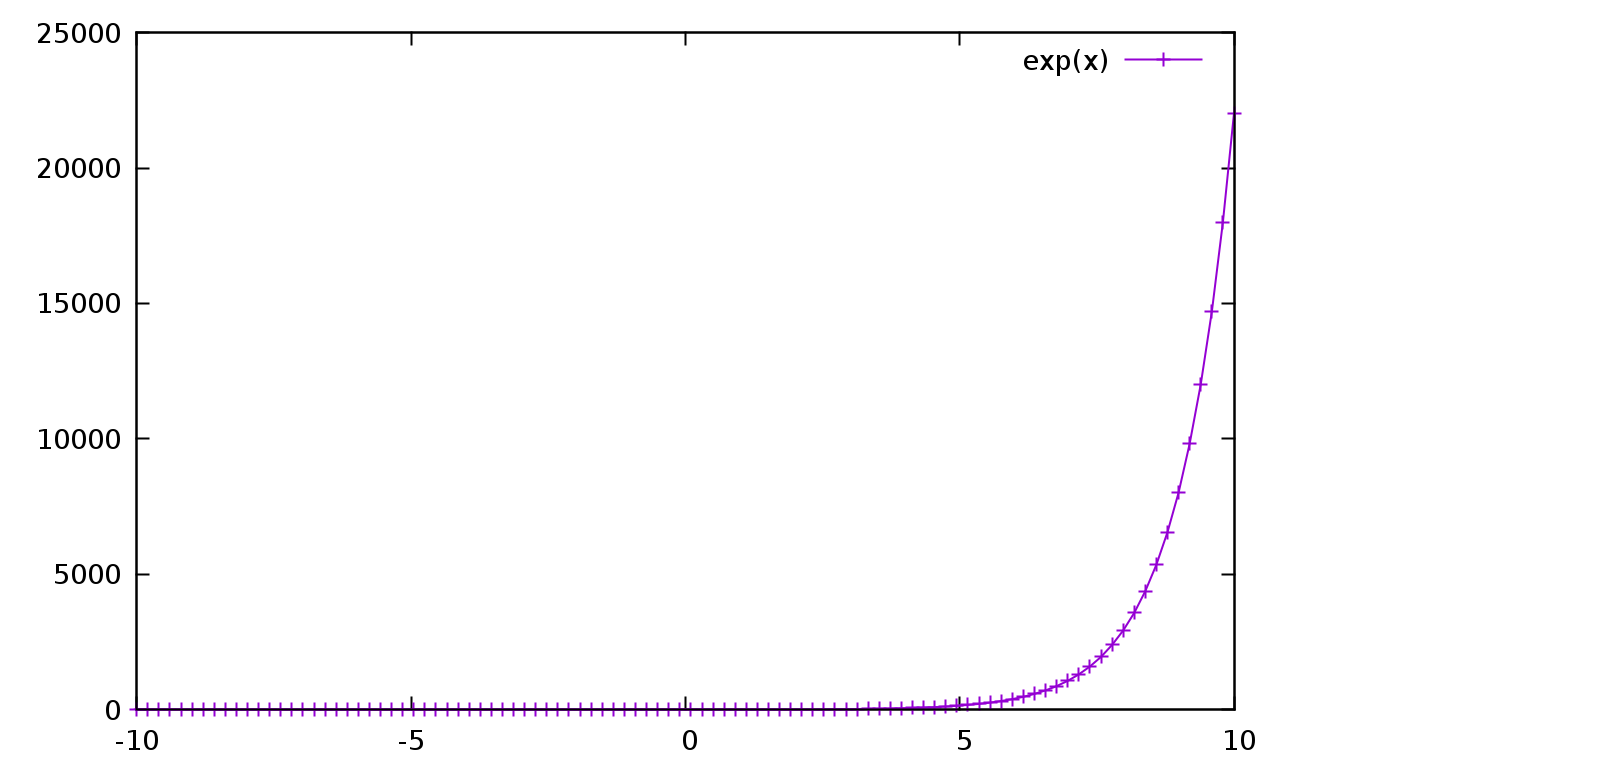
\includegraphics[width=\linewidth]{exponencial.png}
  \caption{Grafica de los valores reales de exp(x)}
\end{figure}
\begin{figure}
  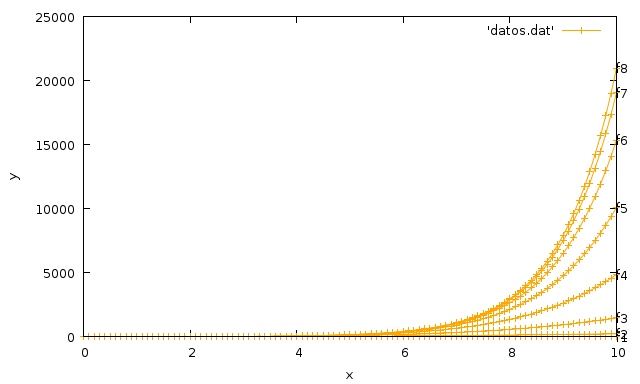
\includegraphics[width=\linewidth]{completo.png}
  \caption{Grafica completa de los valores aproximados de exp(x)}
\end{figure}
\begin{figure}
  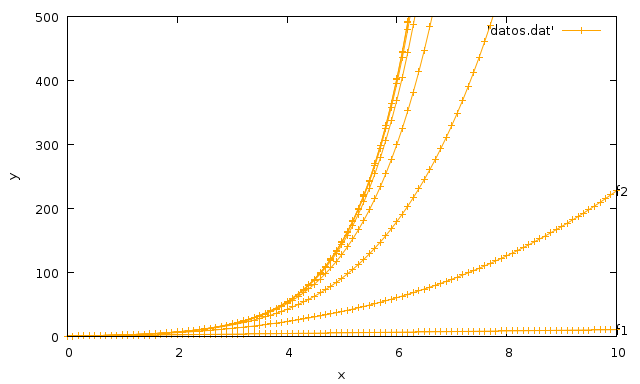
\includegraphics[width=\linewidth]{escala500.png}
  \caption{Grafica hasta y=500 de los valores aproximados de exp(x)}
\end{figure}
\clearpage

\section{Actividad 3: Seno}
\begin{verbatim}
subroutine seno (n, j, fi, fj, sen, signo, potencia, factorial)
	integer, intent (in)      :: n
	double precision, intent (in) :: fi
	integer :: j
	double precision, dimension (10000), intent(out) :: sen
	double precision :: fj, term, partial_sum, signo, potencia, factorial

	
	signo = 1.0d0
	term = fi
	partial_sum = term
	potencia = fi
	factorial = 1
	do j = 1, n
	 fj = dble(j)
	 potencia = fi**(j + 2)
	 factorial = factorial * (j + 1) * (j + 2)
	 signo = signo * (-1.0d0)
	 term = potencia / factorial
	 term = term * signo
	 partial_sum = partial_sum + term
	 sen(j) = partial_sum
	 
	enddo

	 
end subroutine seno
	 

program calculoseno
	double precision, dimension (10000) :: f
	integer :: i, j, n
	double precision, dimension (10000)   :: x
	double precision, dimension (10000) :: sen
	double precision, dimension (10000) :: funcion
	double precision :: fi, fj, term, partial_sum, signo, potencia, factorial
	

     open (1, file = 'senos.dat', status = 'unknown')
	fi = -3.1d0
	do i=1, 60
	write (1,*) fi, fi
	fi = fi + 0.1d0
	
	end do
	write (1,*) ' '
	do n=1, 15, 2
	  fi = -3.1d0
	do i=1, 60
	fi = fi + 0.1d0
	call seno (n, j, fi, fj, sen, signo, potencia, factorial)
	funcion(n) = sen(n)
	write (1,*) fi, funcion(n)

	end do
	write (1,*) ' '
	end do
     close (1)

end program calculoseno
\end{verbatim}
\clearpage
\begin{figure}
  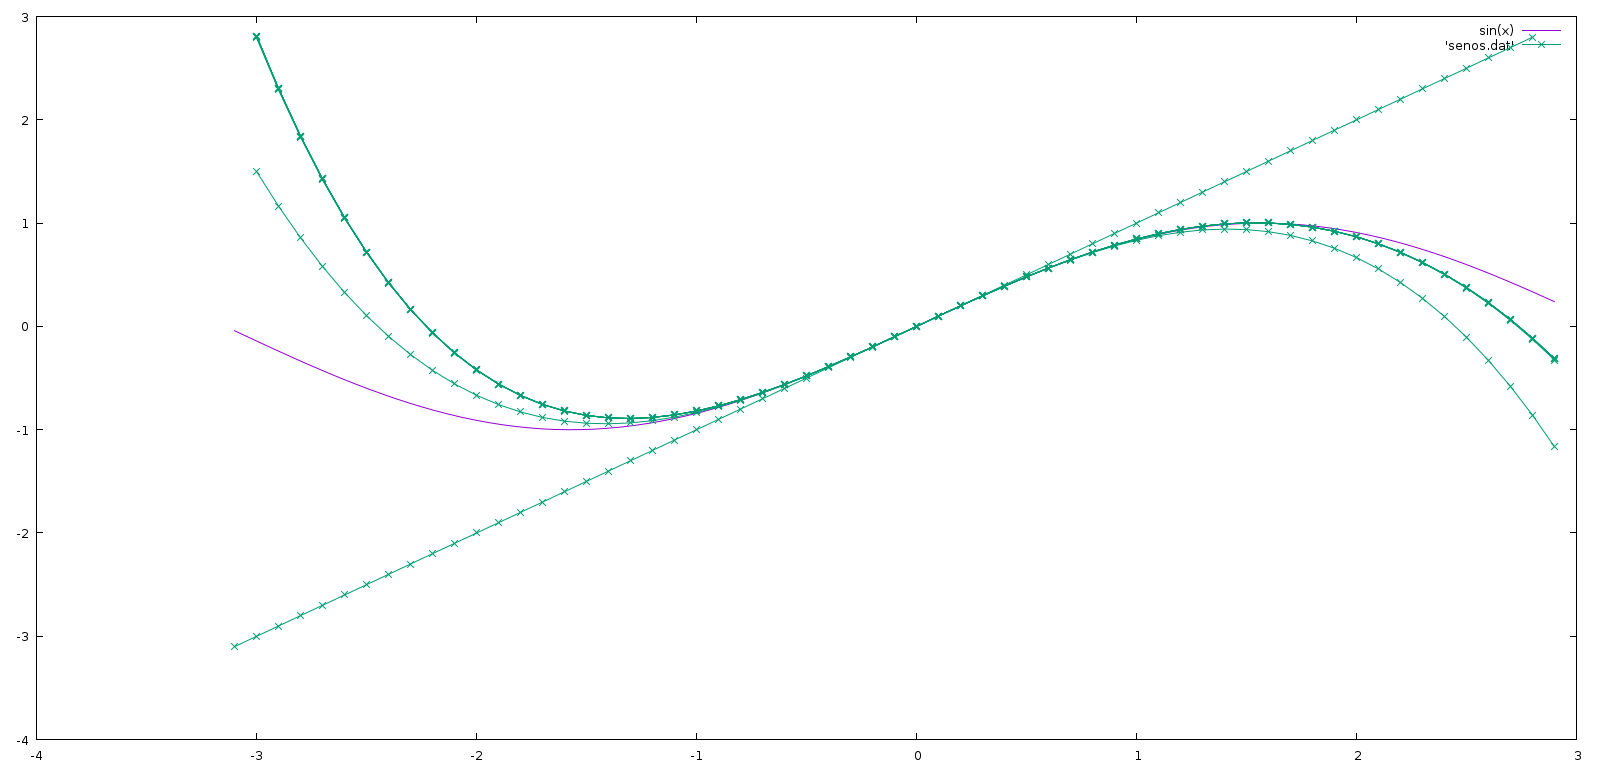
\includegraphics[width=\linewidth]{Senitos.png}
  \caption{Grafica del seno verdadero (color rosa)y las graficas de las aproximaciones}
\end{figure}


\end{document}
